\section{General information}

The project is the making of the course TDT4290 Customer Driven Project. 
Customer driven project is a course held at The Norwegian University of Science and Technology, as mentioned briefly in the preface. 
This course accounts for 15 credits. 
It is a mandatory subject for the 4th year computer science students at IDI. 
The course aims to give the students a real experience with customers in a relevant IT-project. 
This course shall give the students a feel of managing a project in a group. 


All of the different groups is given one customer. 
The customer has put together a project, and to make sure the customer gets what he or she wants, there should be a close relationship with the customer.
Each group also receives an supervisor, which will support and give advice to the group. 


The delivery of the course is a report and a product, and this will be presented to an examiner. 
The report is the most important part of the project, and will contain all the documentation for this project. The course will provide realistic experience in both report writing and product development driven by a customer. 
This will help the students perform better when they are out in real life employment situations.

\section{Structure of report}
You can see the structure of this report in table \ref{tab:structure_of_report}.
\begin{table*}[!h]\centering
\caption{List of all chapters and short description. }
\label{tab:structure_of_report}
\def\arraystretch{1.3}
\begin{tabularx}{\textwidth}{lX} \toprule[1mm]
\textbf{Chapter} & \textbf{Description} \\ \midrule
Chapter 1 & The introduction chapter introduces the problem, and introduces the members and stakeholders of this project.
This chapter also explains the motivation and goals. \\
Chapter 2 &  The preliminary Study chapter describes the work and research done. This chapter describes alternative solutions, and an evaluation these solutions. \\
Chapter 3 &  The planning chapter describes the project plan, the organization, quality assurance and planned workload.  \\

Chapter 4 &  The requirements chapter describes the requirements, both functional and non-functional. It also describes Use cases for the system. \\

Chapter 5 &  The test plan chapter contains the approach for testing with the overall test plan for the project.\\

Chapter 6	 &  The architecture chapter explains the structure of the system, and how it is put together. \\

Chapter 7	 &   The tools and strategy chapter describes the different tools we chose to use for this project.\\

Chapter 8-14 	&  In the sprint chapters the reader can see how the product has developed during the time of the project. This includes planning, architecture, the implementation, testing and evaluation of the sprint. \\

Chapter 15 	 &  The testing chapter describes the different tests. Everything from unit testing to acceptance testing. \\

Chapter 16 	 &  Evaluation chapter includes the team dynamics, risk evaluation, an evaluation of the customer, supervisor and of course the task. \\

Chapter 17 	 &  Conclusion chapter sums up the project, and discusses the solution, and looks at further work. \\

Chapter 18 	 &  The references chapter contains references. \\

Chapter 19 	 &  This chapter contains attachments. \\
\midrule
Appendix 	 &   The appendix contains user manual, installation guide, meeting minutes and more.\\

\bottomrule[1mm]
\end{tabularx}
\end{table*}

\section {Terminology}
\label{sec:terminology}
Since the customer is technically skilled and is used to use Scrum technology, we have adopted his terminology.
After few meetings with the supervisor it was settled that we must present our terminology to prevent from misunderstandings. 
There are also presented product related terminology that will be used in technical parts of this report.

\subsection{Scrum related terms}

\paragraph{User story}
is a short text of user's language of a system that describes user's interaction with the system.

User stories are actually narrative texts that describe an interaction of the user and the system, focusing on the value a user gains from the system.

\paragraph{Epic}
is a large \emph{user story} that will need to be broken down into smaller stories. It is too big to fit into a sprint, or it is unknown as to whether it is too big to fit into a sprint or not.

\paragraph{Task}
If user story is too complex, it can be divided into several tasks. 
Task is then basic unit of problem division.


\paragraph{Milestone}

\subsection{Product related terms}
\paragraph{Client user}
is a participant of concert who wants to actively take part in show and he can download client application.

\paragraph{Server user}
or simply \textbf{Manager} is a person who controls what media should be played on screen made from mobile phone's of users. 
He can also manage other general settings.

\paragraph{End user} is either manager or end client user.

\paragraph{Client} or \textbf{Client side} is an application controlled by client user and provides him opportunity to be part of the screen by displaying figures on his mobile.

\paragraph{Server} or \textbf{Server side} is and application controlled by manager and provides him opportunity to change the media displayed on screen.

\paragraph{Pixel} is a client user's mobile phone under control of manager.


\section{Project and project name}

The customer wants a product to make the audience as a screen on a rock concert. We decided to name the product "digital lighter". We agreed on this name because this product digitalizes the concept from "the old days", where the crowd at a concert held up lighters, to create a special atmosphere. 

\section{Project purpose and concept}

The audience members at a rock concert should be able to download a simple application to their cell phone, and register this through a simple GUI.
Behind the artist on stage there is a screen, with a simple camera on top. 
The camera is taking pictures of the audience. 
At special occasions the audience will be instructed, by the artist, to hold up their phones with the screen towards the stage. 
The mobile is a replacement for the lighter.  

On control a signal the application will fill the entire mobile screen with a single color.
The control signal can as an example say: " all pixels white". 
The signal will be specific for each application.
Each mobile will be a pixel in a larger picture, which will be presented on the big screen. 
What kind of picture the audience can create will depend on the number of people in the audience.   

As a motivation for the audience to hold up their phone, the camera on top of the screen will take pictures of the audience.
In that way the audience can see a reflection of them selves, and see what kind of picture they are creating together.

\section{Project goals}
Goals and objectives are statements that describe what the project will accomplish. The very first step in all projects: business, home, or education, is to define goals and objectives. 
This step defines the projects outcome and the steps required to achieve that outcome. 
It is important to spend sufficient time on this step, or else it can lead to unsuccessful project completion in many different ways. It can push the  a project intro overrun, territory battles, personality clashes, missed milestones, and unhappy customers. 
   
\label{sec:project-goals}

\subsection{Project goals}

\paragraph{Finish the project within the scheduled timetable}
Our goal is be to finished with the project within the given time frame. This means we must do everything possible to drive the project to the end and stay on time. Remember to avoid guessing in the planning of the scope.

\paragraph{Finish the project within the specified guidelines}
Another goal is to make sure we are meeting the customer's needs. We want "wow" the customer! 
This can be done simply by finishing the project with the specifics the customer really wanted. The best way to solidify this is to verify your accomplishment by customer hand off and close down.

\subsection{Group goals}
\paragraph{Receive a good grade}
Getting a good grade is important because it says something about what you have learned in this course. 
This is relevant in terms of what job we might get when we have graduated. It also shows an employer that we can work hard. 
\paragraph{Receive a good recommendation from customer/supervisor}
If we work really hard, and impress the supervisor and the customer it would be nice to get a recommendation. This would be a bonus for our CV.


\paragraph{Do the best we can with what we have been given}
There is no such thing as a perfect project.
Some projects run up against major odds and hurdles, and project goals were met because they did their best with what came their way. One of ours goals is of course to do the best with what we have been given.


\subsection{Personal goals}
\paragraph{Agnethe}

My personal goal is to learn about group dynamics and collaboration. Another goal is learn more about writing reports, because it is important to get some experience before writing the masters report. One of my goals is also to  satisfy our customer, and maybe get a good recommendation. It is also a great chance that I might work as an IT-consultant, and I want to learn as much as possible about this profession. I also  get better at holding presentations, because there will always be another presentation to hold. I also want to learn as much as possible about android and mobile development.

\paragraph{Jan}
\paragraph{Milos}
\paragraph{Tomas}
I have chosen NTNU university for my exchange studies because of this class. 
I was expecting to improve my soft-skills, software engineering knowledge and also my written and spoken English and to be treated like in real project.
As this class has already started, I can add to my personal goals also learning Java programming language,
Android platform development and improving my skills concerning image processing.

\section{Stakeholders}

The stakeholders in this project is any person or organization, which has some interest or is affected by this project. Together they construct the different restrictions and goals for the project. 
You can see the organization chart in figure \ref{img:organization_chart}.

\begin{figure}[!h]
    \begin{center}
    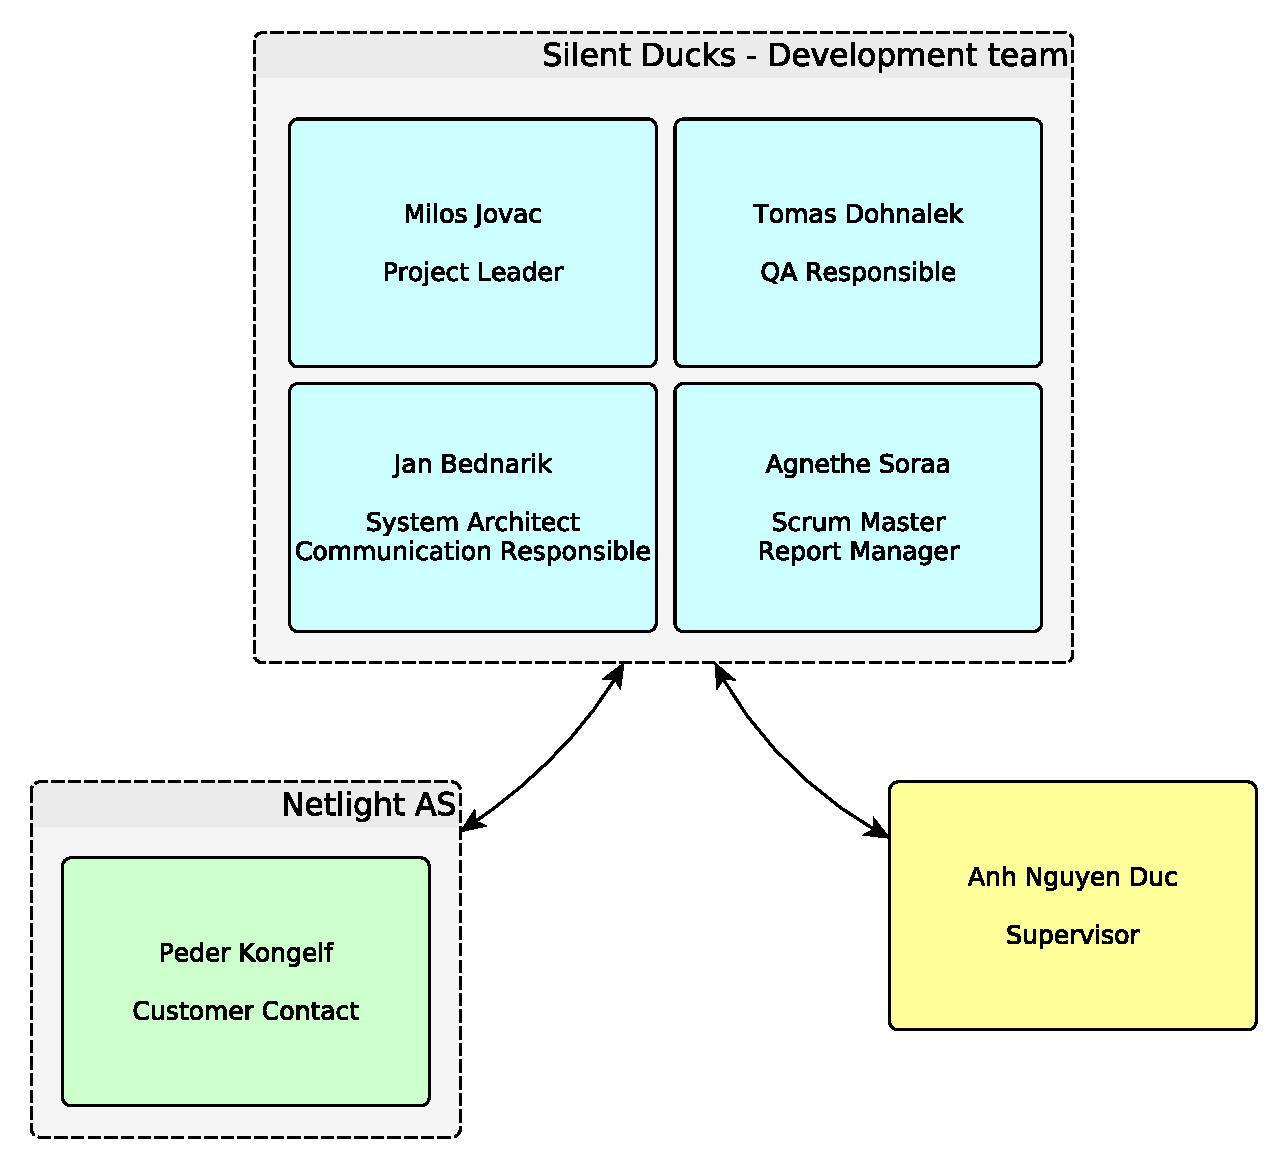
\includegraphics[scale=0.4]{images/organization_chart.pdf}
    \caption{Chart depicting team organization and its stakeholders.}
    \label{img:organization_chart}
    \end{center}
\end{figure}

\subsection{Customer}
Netlight AS is a consulting company engaged in IT and management. Their field of expertise is within IT management, IT governance, IT-strategy, IT-organization and IT-research. They deliver unique solutions based on their customers requirements. They operates throughout Europe with offices in Stockholm, Oslo, London, Munich and Helsinki. The company was founded at 1999 and employs to 500 employees. 
\subsubsection{Customer contact}
Peder Kongelf will be our contact person in Netlight. We will have weekly meetings with him to make sure the project is going in the right direction, and of course get opportunities to ask questions. This way we will get a better understanding of the project.

\subsection{Development team}
 The development team's role is, first of all, to meet all requirements presented by the customer and IDI. We are responsible for development of the project. We are also responsible for writing all the documentation for this course.  Our interest in the project is to receive experience with new technologies and project management, as well as to receive satisfactory grading. You can read about personal goals in section \ref{sec:project-goals}. 
 
 The project was intended for 5-7 students,but we are only 4 members in our team. This will, in some way, affect what the team can manage towards what was expected when the project was put together.

\subsection{Supervisor}

Anh Nguyen Doc is the supervisor assigned to this project from The Department of Computer and Information Science. The main responsibility of the team's supervisor is to overview the whole project and discuss the work done together with the future plans. Since the decisions and suggestions of this person are of the great importance the team agreed on holding the supervisor meetings once a week. The team should prepare the meeting minutes document and send it to the supervisor before the next meeting.


Of course the interest from the university in general is to provide some real experience to the students, and prepare them for the business world.


\subsection{End users}
Is a everyday person who uses the end product. Our plan is to release the product on the application store for Android. That way we can get feedback from someone other than supervisor and customer. 
\subsection{Stakeholder summary}
You can see the table with email contacts in table \ref{tab:stakeholders_summary}.

\begin{table*}[!h]\centering
\caption{List of all stakeholders with their role and email contact. }
\label{tab:stakeholders_summary}
\def\arraystretch{1.15}
\begin{tabular}{lll}
\toprule[1mm]
\textbf{Person} & \textbf{Email} & \textbf{Role}\\
\midrule
Peder Kongelf & peder.kongelf@gmail.com  & Customer\\
\midrule
Anh Nguyen Doc	 & anhn@idi.ntnu.no & Supervisor \\
\midrule
Milos Jovac &  milosjovac@gmail.com & Team member  \\
Jan Bednarik &  ja.bedna1@gmail.com & Team member\\
Agnethe Soraa & agnethes0raa@gmail.com & Team member  \\
Tomas Dohnalek & dohnto@gmail.com & Team member \\
\bottomrule[1mm]

\end{tabular}
\end{table*}